\special{! TeXDict begin /landplus90{true}store end }

\documentclass[xga]{xdvislides}
\usepackage[landscape]{geometry}
\usepackage{graphics}
\usepackage{graphicx}
\usepackage{colordvi}
\usepackage{multirow}
\usepackage[normalem]{ulem}

\usepackage{fancyvrb}
\fvset{fontfamily=courier,commandchars=\\\{\}}

\begin{document}
\setfontphv

%%% Headers and footers
\lhead{\slidetitle}                               % default:\lhead{\slidetitle}
\chead{CS615 - Aspects of System Administration}% default:\chead{\relax}
\rhead{Slide \thepage}                       % default:\rhead{\sectiontitle}
\lfoot{\Gray{SMTP, HTTPS / TLS}}% default:\lfoot{\slideauthor}
\cfoot{\relax}                               % default:\cfoot{\relax}
\rfoot{\Gray{\today}}

\newcommand{\smallish}{\fontsize{16}{16}\selectfont}

\vspace*{\fill}
\begin{center}
	\Hugesize
		CS615 - Aspects of System Administration\\ [1em]
		SMTP, HTTPS / TLS\\ [1em]
	\hspace*{5mm}\blueline\\ [1em]
	\Normalsize
		Department of Computer Science\\
		Stevens Institute of Technology\\
		Jan Schaumann\\
		\verb+jschauma@stevens.edu+\\
		\verb+https://www.cs.stevens.edu/~jschauma/615/+
\end{center}
\vspace*{\fill}

\subsection{Email... still popular}
Bad news, everybody: Slack has not yet replaced email.

\subsection{Email... still popular}
Good news, everybody: Slack has not yet replaced email. (And it's not going to.)
\\

\begin{itemize}
	\item {\bf 4.6 billion} - number of email accounts.
	\item {\bf 269 billion} - Average number of email messages per day. \\
		That's 3.1 million emails {\em per second}.
	\item {\bf 121} - Average number of emails an office worker receives.
	\item {\bf 42} - Percentage of Americans that check their email in the bathroom.
	\item {\bf 18} - Percentage of Americans that check their email while driving.
	\item {\bf $>$70} - Percentage of emails that are Spam.
\end{itemize}

\subsection{Sending...}
\begin{verbatim}
# tcpdump -i xennet0 -w /tmp/t.out port not 22 2>/dev/null &
# mail -s "CS615 - SMTP Exercise" jschauma@stevens.edu -f jschauma@stevens.edu
Hello,

SMTP is so simple!

-Jan
.
EOT
# fg
tcpdump -i xennet0 -w /tmp/t.out port not 22 2>/dev/null
^C
\end{verbatim}


\subsection{Sending...}
\begin{verbatim}
# tail -5 /var/log/maillog
Mar 17 19:07:46 ip-10-225-79-205 postfix/pickup[1937]:
        981302FFB4: uid=0 from=<jschauma@stevens.edu>
Mar 17 19:07:46 ip-10-225-79-205 postfix/cleanup[2252]:
        981302FFB4: message-id=<20180317190746.981302FFB4@ip-10-225-79-205.ec2.internal>
Mar 17 19:07:46 ip-10-225-79-205 postfix/qmgr[1662]:
        981302FFB4: from=<jschauma@stevens.edu>, size=381, nrcpt=1 (queue active)
Mar 17 19:07:47 ip-10-225-79-205 postfix/smtp[2285]:
        981302FFB4: to=<jschauma@stevens.edu>, relay=spamfilter01.stevens.edu[155.246.14.37]:25,
        delay=0.42, delays=0.02/0/0.17/0.23, dsn=2.0.0, status=sent (250 Ok: queued as 17A35227E1D4)
Mar 17 19:07:47 ip-10-225-79-205 postfix/qmgr[1662]:
        981302FFB4: removed
\end{verbatim}

\subsection{Sending...}
\begin{verbatim}
# tcpdump -t -r /tmp/t.out port 53
IP 10.225.79.205.65530 > 172.16.0.23.53: 35305+ MX? stevens.edu. (29)
IP 172.16.0.23.53 > 10.225.79.205.65530: 35305 2/0/0
        MX spamfilter02.stevens.edu. 20, MX spamfilter01.stevens.edu. 10 (87)
IP 10.225.79.205.65529 > 172.16.0.23.53: 1856+ A? spamfilter01.stevens.edu. (42)
IP 172.16.0.23.53 > 10.225.79.205.65529: 1856 1/0/0 A 155.246.14.37 (58)
IP 10.225.79.205.65528 > 172.16.0.23.53: 63422+ AAAA? spamfilter01.stevens.edu. (42)
IP 172.16.0.23.53 > 10.225.79.205.65528: 63422 0/1/0 (113)
IP 10.225.79.205.65527 > 172.16.0.23.53: 55675+ A? spamfilter02.stevens.edu. (42)
IP 172.16.0.23.53 > 10.225.79.205.65527: 55675 1/0/0 A 155.246.248.24 (58)
IP 10.225.79.205.65526 > 172.16.0.23.53: 41719+ AAAA? spamfilter02.stevens.edu. (42)
IP 172.16.0.23.53 > 10.225.79.205.65526: 41719 0/1/0 (113)
\end{verbatim}

\subsection{Sending...}
\begin{verbatim}
# host -t mx stevens.edu
stevens.edu mail is handled by 20 spamfilter02.stevens.edu.
stevens.edu mail is handled by 10 spamfilter01.stevens.edu.
# host spamfilter01.stevens.edu
spamfilter01.stevens.edu has address 155.246.14.37
# host spamfilter02.stevens.edu
spamfilter02.stevens.edu has address 155.246.248.24
#
\end{verbatim}

\subsection{Sending...}
\smallish
\begin{verbatim}
IP 10.225.79.205.65531 > 155.246.14.37.25: Flags [S], seq 3766385453
IP 155.246.14.37.25 > 10.225.79.205.65531: Flags [S.], seq 2325444199, ack 3766385454
IP 10.225.79.205.65531 > 155.246.14.37.25: Flags [.], ack 1
IP 155.246.14.37.25 > 10.225.79.205.65531: Flags [P.], seq 1:72
        SMTP: 220 spamfilter01.stevens.edu ESMTP (fe32969a29a5f461e53bf93b18c8fdb5)
IP 10.225.79.205.65531 > 155.246.14.37.25: Flags [P.], seq 1:37, ack 72
        SMTP: EHLO ip-10-225-79-205.ec2.internal
IP 155.246.14.37.25 > 10.225.79.205.65531: Flags [.], ack 37, win 114
IP 155.246.14.37.25 > 10.225.79.205.65531: Flags [P.], seq 72:244, ack 37
        SMTP: 250-spamfilter01.stevens.edu Hello ec2-54-225-8-178.compute-1.amazonaws.com
        [54.225.8.178], pleased to meet you
IP 10.225.79.205.65531 > 155.246.14.37.25: Flags [P.], seq 37:118, ack 244
        SMTP: MAIL FROM:<jschauma@stevens.edu> SIZE=381
IP 155.246.14.37.25 > 10.225.79.205.65531: Flags [P.], seq 244:282, ack 118
        SMTP: 250 Sender <jschauma@stevens.edu> OK
IP 10.225.79.205.65531 > 155.246.14.37.25: Flags [.], ack 282, win 4197
IP 155.246.14.37.25 > 10.225.79.205.65531: Flags [P.], seq 282:369, ack 118
        SMTP: 250 Recipient <jschauma@stevens.edu> OK
IP 10.225.79.205.65531 > 155.246.14.37.25: Flags [P.], seq 118:508, ack 369
        SMTP: Received: by ip-10-225-79-205.ec2.internal (Postfix, from userid 0)
IP 155.246.14.37.25 > 10.225.79.205.65531: Flags [P.], seq 369:401, ack 508
        SMTP: 250 Ok: queued as 17A35227E1D4
IP 155.246.14.37.25 > 10.225.79.205.65531: Flags [FP.], seq 401:500, ack 508
        SMTP: 221 spamfilter01.stevens.edu Goodbye ec2-54-225-8-178.compute-1.amazonaws.com, closing connection
\end{verbatim}
\Normalsize

\subsection{SMTP Codes}
SMTP codes consist of three digits in five classes:
\begin{itemize}
	\item {\bf 1xx} --  Mail server has accepted the command, but does not yet
		take any action. A confirmation message is required.
	\item {\bf 2xx} --  Mail server has completed the task successfully
		without errors.
	\item {\bf 3xx} --  Mail server has understood the request, but requires
		further information to complete it.
	\item {\bf 4xx} --  Mail server has encountered a temporary failure. If
		the command is repeated without any change, it might be
		completed. Try again, it may help!
	\item {\bf 5xx} --  Mail server has encountered a fatal error. Your
		request can't be processed.
\end{itemize}

\subsection{Sending...}
\begin{center}
	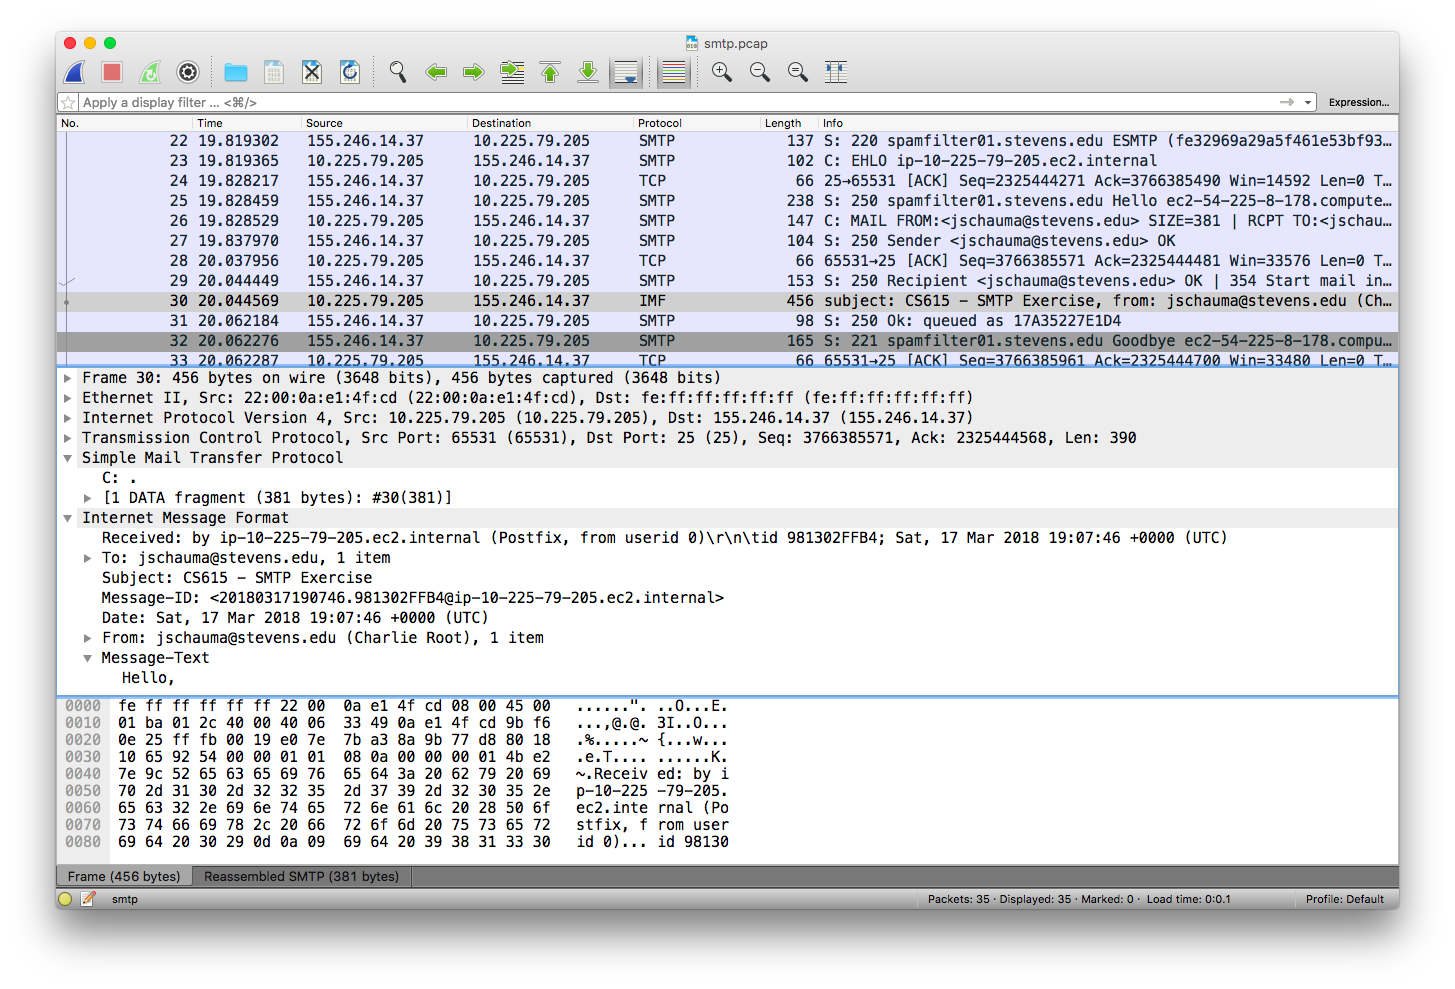
\includegraphics[scale=0.35]{pics/wireshark-smtp.eps}
\end{center}

\subsection{Sending...}
\begin{Verbatim}
$ telnet 155.246.14.37 25
Trying 155.246.14.37...
Connected to spamfilter01.stevens.edu.
Escape character is '^]'.
220 spamfilter01.stevens.edu ESMTP (fe32969a29a5f461e53bf93b18c8fdb5)
\textbf{EHLO ip-10-235-167-232.ec2.internal}
250-spamfilter01.stevens.edu Hello ec2-54-205-68-41.compute-1.amazonaws.com [54.205.68.41],
        pleased to meet you
250-SIZE 50000000
250-PIPELINING
250-8BITMIME
250 HELP
\textbf{MAIL FROM: <jschauma@stevens.edu> SIZE=380}
250 Sender <jschauma@stevens.edu> OK
\textbf{RCPT TO: <jschauma@stevens.edu>}
250 Recipient <jschauma@stevens.edu> OK
\end{Verbatim}

\subsection{Sending...}
\begin{Verbatim}
\textbf{DATA}
354 Start mail input; end with <CRLF>.<CRLF>
\textbf{Received: by ip-10-225-79-205.ec2.internal (Postfix, from userid 0)}
\textbf{        id 981302FFB4; Sat, 17 Mar 2018 19:07:46 +0000 (UTC)}
\textbf{To: jschauma@stevens.edu}
\textbf{Subject: CS615 - SMTP Exercise}
\textbf{Message-Id: <20180317190746.981302FFB4@ip-10-225-79-205.ec2.internal>}
\textbf{Date: Sat, 17 Mar 2018 19:07:46 +0000 (UTC)}
\textbf{From: jschauma@stevens.edu (Charlie Root)}

\textbf{Hello,}

\textbf{SMTP is so simple!}

\textbf{-Jan}
\textbf{.}
250 Ok: queued as 17A35227E1D4
\end{Verbatim}

\subsection{Receiving...}
\small
\begin{verbatim}
IP 155.246.14.12.49256 > 166.84.7.99.25: Flags [S], seq 2581060655
IP 166.84.7.99.25 > 155.246.14.12.49256: Flags [S.], seq 567627508, ack 2581060656
IP 155.246.14.12.49256 > 166.84.7.99.25: Flags [.], ack 1
IP 166.84.7.99.25 > 155.246.14.12.49256: Flags [P.], seq 1:41, ack 1
IP 155.246.14.12.49256 > 166.84.7.99.25: Flags [.], ack 41
IP 155.246.14.12.49256 > 166.84.7.99.25: Flags [P.], seq 1:25, ack 41
IP 166.84.7.99.25 > 155.246.14.12.49256: Flags [P.], seq 41:174, ack 25,
IP 155.246.14.12.49256 > 166.84.7.99.25: Flags [P.], seq 25:35, ack 174
IP 166.84.7.99.25 > 155.246.14.12.49256: Flags [P.], seq 174:204, ack 35
IP 155.246.14.12.49256 > 166.84.7.99.25: Flags [P.], seq 35:334, ack 204
IP 166.84.7.99.25 > 155.246.14.12.49256: Flags [P.], seq 204:362, ack 334
IP 155.246.14.12.49256 > 166.84.7.99.25: Flags [P.], seq 334:484, ack 362
IP 166.84.7.99.25 > 155.246.14.12.49256: Flags [P.], seq 362:612, ack 484
IP 155.246.14.12.49256 > 166.84.7.99.25: Flags [P.], seq 484:553, ack 612
IP 166.84.7.99.25 > 155.246.14.12.49256: Flags [P.], seq 612:793, ack 553
IP 155.246.14.12.49256 > 166.84.7.99.25: Flags [P.], seq 553:734, ack 793
IP 166.84.7.99.25 > 155.246.14.12.49256: Flags [P.], seq 793:910, ack 734
IP 155.246.14.12.49256 > 166.84.7.99.25: Flags [.], seq 734:2182, ack 910
IP 155.246.14.12.49256 > 166.84.7.99.25: Flags [.], seq 2182:3630, ack 910
IP 155.246.14.12.49256 > 166.84.7.99.25: Flags [P.], seq 3630:3955, ack 910
IP 166.84.7.99.25 > 155.246.14.12.49256: Flags [.], ack 3630
IP 166.84.7.99.25 > 155.246.14.12.49256: Flags [.], ack 3955
IP 166.84.7.99.25 > 155.246.14.12.49256: Flags [P.], seq 910:1011, ack 3955
IP 155.246.14.12.49256 > 166.84.7.99.25: Flags [P.], seq 3955:4008, ack 1011
IP 166.84.7.99.25 > 155.246.14.12.49256: Flags [P.], seq 1011:1064, ack 4008
IP 155.246.14.12.49256 > 166.84.7.99.25: Flags [F.], seq 4008, ack 1064
IP 166.84.7.99.25 > 155.246.14.12.49256: Flags [.], ack 4009
IP 166.84.7.99.25 > 155.246.14.12.49256: Flags [F.], seq 1064, ack 4009
IP 155.246.14.12.49256 > 166.84.7.99.25: Flags [.], ack 1065
\end{verbatim}
\Normalsize

\subsection{Receiving...}
\begin{center}
	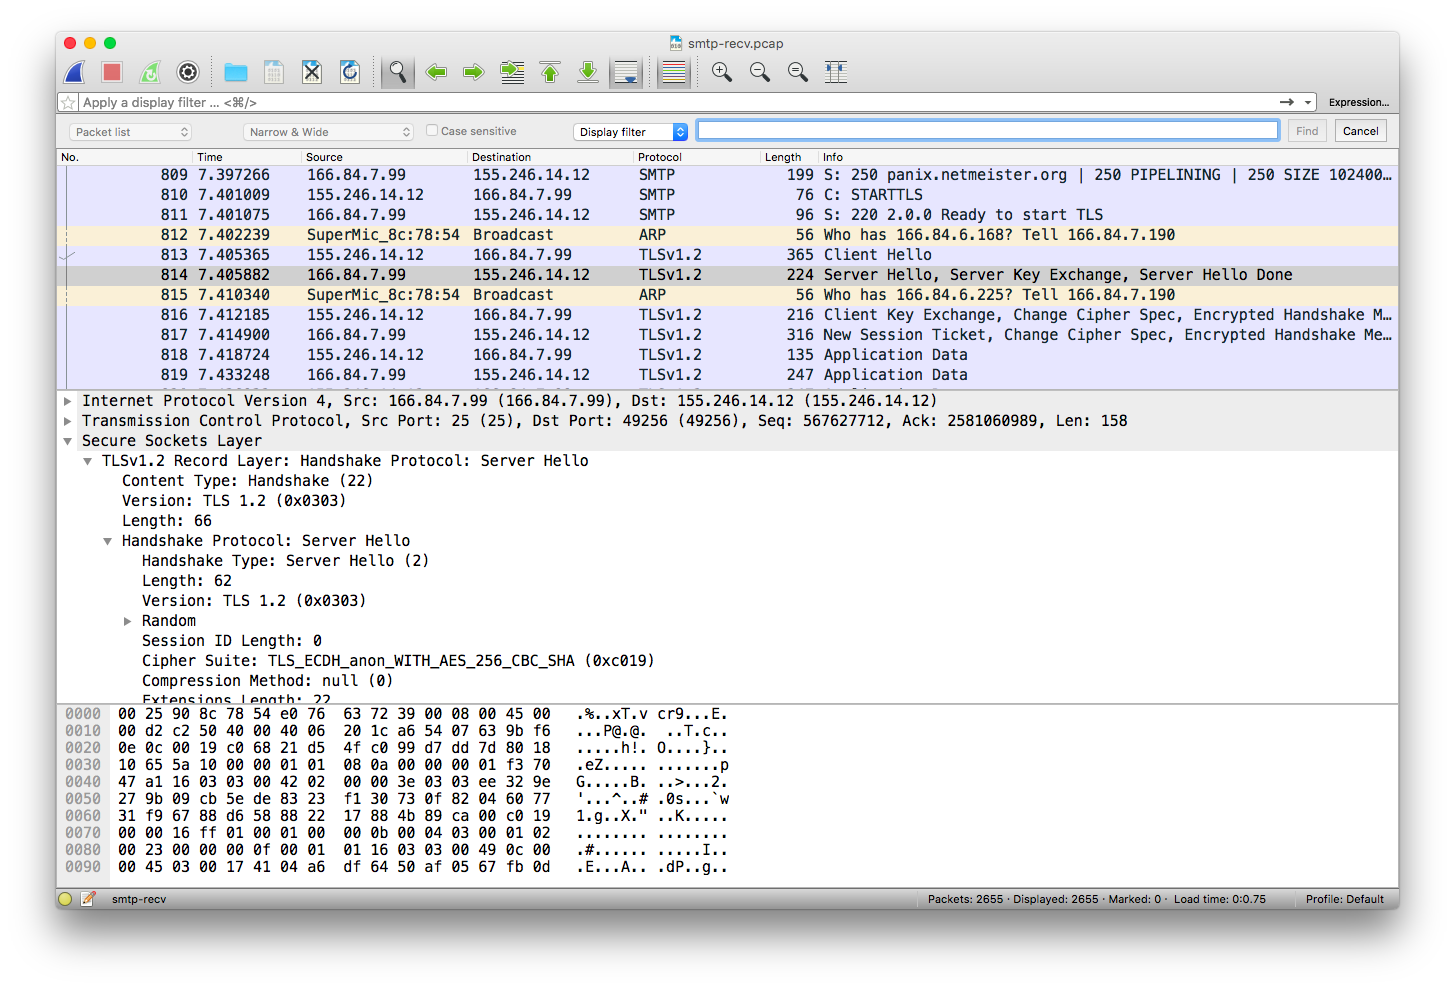
\includegraphics[scale=0.35]{pics/wireshark-smtp-tls.eps}
\end{center}


\subsection{Receiving...}
\smallish
\begin{verbatim}
$ tail -f /var/log/maillog
postfix/smtpd[7933]: connect from nexus.stevens.edu[155.246.14.12]
postfix/smtpd[7933]: Anonymous TLS connection established from
        nexus.stevens.edu[155.246.14.12]: TLSv1.2 with cipher AECDH-AES256-SHA (256/256 bits)
postfix/smtpd[7933]: 6D2A1650D8: client=nexus.stevens.edu[155.246.14.12]
postfix/cleanup[19825]: 6D2A1650D8: message-id=<943d7213a0a54930a35db5c0b0e94de2@exchng03.campus.stevens-tech.edu>
postfix/cleanup[19825]: 6D2A1650D8: resent-message-id=<20180317192418.1B4111814A1@nexus.stevens.edu>
postfix/qmgr[1885]: 6D2A1650D8: from=<jschauma@stevens.edu>, size=3456, nrcpt=1 (queue active)
postfix/smtpd[7933]: disconnect from nexus.stevens.edu[155.246.14.12]
postfix/pickup[9347]: DA65C65140: uid=1004 from=<jschauma@stevens.edu>
postfix/cleanup[19825]: DA65C65140: message-id=<943d7213a0a54930a35db5c0b0e94de2@exchng03.campus.stevens-tech.edu>
postfix/cleanup[19825]: DA65C65140: resent-message-id=<20180317192418.1B4111814A1@nexus.stevens.edu>
postfix/qmgr[1885]: DA65C65140: from=<jschauma@stevens.edu>, size=3803, nrcpt=1 (queue active)
postfix/local[9885]: DA65C65140: to=<jschauma@netmeister.org>, relay=local,
        delay=0.22, delays=0.09/0/0/0.13, dsn=2.0.0,
        status=sent (delivered to command: /usr/pkg/bin/procmail)
postfix/qmgr[1885]: DA65C65140: removed
\end{verbatim}
\Normalsize


\subsection{Receiving...}
\begin{verbatim}
Date: Sat, 17 Mar 2018 19:07:46 +0000
From: Jan Schaumann <jschauma@stevens.edu>
To: Jan Schaumann <jschauma@stevens.edu>
Subject: CS615 - SMTP Exercise

Hello,

SMTP is so simple!

-Jan
\end{verbatim}

\subsection{Anatomy of an email message}
An email consists of:
\begin{itemize}
	\item mandatory headers (such as "From ", "Delivered-To: ", ...)
	\item optional headers (such as "From: ", "To: ", "Subject: ", ...)
	\item the body of the message
	\begin{itemize}
		\item content independent of SMTP
		\item Multipurpose Internet Mail Extensions (MIME) enables non-ascii, multipart, encodings, ...
	\end{itemize}
\end{itemize}


\subsection{Receiving...}
\smallish
\begin{verbatim}
From jschauma@stevens.edu  Sat Mar 17 15:24:18 2018                                                 
Received: by panix.netmeister.org (Postfix, from userid 1004)
        id DA65C65140; Sat, 17 Mar 2018 15:24:18 -0400 (EDT)
Received: from nexus.stevens.edu (nexus.stevens.edu [155.246.14.12])
        (using TLSv1.2 with cipher AECDH-AES256-SHA (256/256 bits))
        (No client certificate requested)
        by panix.netmeister.org (Postfix) with ESMTPS id 6D2A1650D8
        for <jschauma@netmeister.org>; Sat, 17 Mar 2018 15:24:18 -0400 (EDT)
Received: from exchng01.campus.stevens-tech.edu (exchng01.campus.stevens-tech.edu [155.246.14.21])
        by nexus.stevens.edu (Postfix) with ESMTPS id 1B4111814A1
        for <jschauma@netmeister.org>; Sat, 17 Mar 2018 15:24:18 -0400 (EDT)
Received: from exchng04.campus.stevens-tech.edu (2002:9bf6:f826::9bf6:f826) by
        exchng01.campus.stevens-tech.edu (2002:9bf6:e16::9bf6:e16) with Microsoft
        SMTP Server (TLS) id 15.0.1263.5; Sat, 17 Mar 2018 15:24:17 -0400
Received: from exchng03.campus.stevens-tech.edu (155.246.248.36) by
        exchng04.campus.stevens-tech.edu (155.246.248.39) with Microsoft SMTP Server
        (TLS) id 15.0.1263.5; Sat, 17 Mar 2018 15:24:17 -0400
Received: from exchng03.campus.stevens-tech.edu ([::1]) by
        exchng03.campus.stevens-tech.edu ([fe80::599a:f128:d1b3:4ce7%12]) with
        Microsoft SMTP Server id 15.00.1263.000; Sat, 17 Mar 2018 15:24:17 -0400
From: Jan Schaumann <jschauma@stevens.edu>
To: Jan Schaumann <jschauma@stevens.edu>
Subject: CS615 - SMTP Exercise
Date: Sat, 17 Mar 2018 19:07:46 +0000
\end{verbatim}
\Normalsize

\subsection{SMTP is a Simple Mail Transfer Protocol.}

\begin{itemize}
	\item TCP port 25
	\item DNS MX records
	\item mail may be relayed or processed by many servers in transit
	\item transport is in clear text
	\item STARTTLS may provide (opportunistic) transport encryption
	\item SPAM controls may include DNS lookups, bayesian scoring, ...
	\item authenticity not guaranteed (more on that in a minute)
\end{itemize}

\subsection{The Mail System}
Divided into:
\begin{itemize}
	\item {\em Mail User Agent} or MUA, such as {\tt mutt(1)}, {\em Mail.app}, {\em Outlook}, a browser (ugh) ...
	\item {\em Mail Transfer Agent} or MTA, such as {\em postfix},
		{\em sendmail}, {\em qmail}, ...
	\item {\em Mail Delivery Agent} or MDA, such as {\em procmail}
	\item {\em Access Agent} providing access via {\em POP}, {\em IMAP} etc.
\end{itemize}
\vspace{.5in}
In addition, many MUAs nowadays interpret HTML:
\begin{itemize}
	\item browser now the most common MUA
	\item facilitates phishing (via link obscuring, logos etc.)
	\item facilitates tracking (via beacons, cookies)
\end{itemize}

\subsection{Authenticity and SPAM}
\vspace*{\fill}
\begin{center}
	
\includegraphics[scale=1.0]{pics/spam.eps} \\
	{\tt https://youtu.be/anwy2MPT5RE}
\end{center}
\vspace*{\fill}

\subsection{Relaying mail}
\begin{verbatim}
220 spamfilter01.stevens.edu ESMTP (fe32969a29a5f461e53bf93b18c8fdb5)
HELO localhost
250 spamfilter01.stevens.edu Hello ec2-54-225-8-178.compute-1.amazonaws.com
        [54.225.8.178], pleased to meet you
MAIL FROM: <leaks@whitehouse.gov>
250 Sender <leaks@whitehouse.gov> OK
RCPT TO: <mueller@fbi.gov>
550 No such domain at this location
\end{verbatim}

\subsection{Authenticity}
\smallish
\begin{verbatim}
220 spamfilter01.stevens.edu ESMTP (fe32969a29a5f461e53bf93b18c8fdb5)
HELO localhost
250 spamfilter01.stevens.edu Hello ec2-54-225-8-178.compute-1.amazonaws.com
        [54.225.8.178], pleased to meet you
MAIL FROM: <barack@obama.org>
250 Sender <barack@obama.org> OK
RCPT TO: <jschauma@stevens.edu>
250 Recipient <jschauma@stevens.edu> OK
DATA
354 Start mail input; end with <CRLF>.<CRLF>
From: "Barack Obama" <barack@obama.org>
To: "Jan Schaumann" <jschauma@stevens.edu>
Subject: Friday

Yo,

Party at my house.
BYOB.

-B
.
250 Ok: queued as DB6C9227E1D4
\end{verbatim}
\Normalsize

\subsection{Authenticity}
\begin{verbatim}
Date: Sun, 18 Mar 2018 20:44:42 +0000
From: Barack Obama <barack@obama.org>
To: Jan Schaumann <jschauma@stevens.edu>
Subject: Friday

Yo,

Party at my house.
BYOB.

-B
\end{verbatim}

\subsection{Receiving...}
\smallish
\begin{verbatim}
$ tail -f /var/log/maillog
postfix/smtpd[7933]: connect from nexus.stevens.edu[155.246.14.12]
postfix/smtpd[7933]: Anonymous TLS connection established from
        nexus.stevens.edu[155.246.14.12]: TLSv1.2 with cipher AECDH-AES256-SHA (256/256 bits)
postfix/smtpd[7933]: 6D2A1650D8: client=nexus.stevens.edu[155.246.14.12]
postfix/cleanup[19825]: 6D2A1650D8: message-id=<943d7213a0a54930a35db5c0b0e94de2@exchng03.campus.stevens-tech.edu>
postfix/cleanup[19825]: 6D2A1650D8: resent-message-id=<20180317192418.1B4111814A1@nexus.stevens.edu>
postfix/qmgr[1885]: 6D2A1650D8: from=<jschauma@stevens.edu>, size=3456, nrcpt=1 (queue active)
postfix/smtpd[7933]: disconnect from nexus.stevens.edu[155.246.14.12]
spamd[10470]: spamd: connection from localhost [::1]:59757 to port 783, fd 5
spamd[10470]: spamd: processing message <943d7213a0a54930a35db5c0b0e94de2@exchng03.campus.stevens-tech.edu>
        aka <20180317192418.1B4111814A1@nexus.stevens.edu> for spamd:1004
postfix/pipe[9461]: 6D2A1650D8: to=<jschauma@netmeister.org>,
        relay=spamassassin, delay=0.59, delays=0.16/0/0/0.43,
        dsn=2.0.0, status=sent (delivered via spamassassin service)
postfix/qmgr[1885]: 6D2A1650D8: removed
postfix/pickup[9347]: DA65C65140: uid=1004 from=<jschauma@stevens.edu>
postfix/cleanup[19825]: DA65C65140: message-id=<943d7213a0a54930a35db5c0b0e94de2@exchng03.campus.stevens-tech.edu>
postfix/cleanup[19825]: DA65C65140: resent-message-id=<20180317192418.1B4111814A1@nexus.stevens.edu>
postfix/qmgr[1885]: DA65C65140: from=<jschauma@stevens.edu>, size=3803, nrcpt=1 (queue active)
postfix/local[9885]: DA65C65140: to=<jschauma@netmeister.org>, relay=local,
        delay=0.22, delays=0.09/0/0/0.13, dsn=2.0.0,
        status=sent (delivered to command: /usr/pkg/bin/procmail)
postfix/qmgr[1885]: DA65C65140: removed
\end{verbatim}
\Normalsize


\subsection{Authenticity and SPAM}
\begin{verbatim}
x-barracuda-spam-score: 6.04
x-barracuda-spam-status: No, SCORE=6.04 using per-user scores of
        TAG_LEVEL=1000.0 QUARANTINE_LEVEL=1000.0 KILL_LEVEL=1000.0
        tests=HELO_LOCALHOST, HELO_LOCALHOST_2, MISSING_DATE, MISSING_MID
x-barracuda-spam-report: Code version 3.2, rules version 3.2.3.49089    Rule
        breakdown below  pts rule name description ----
        ------------------------------------------------------------------------
        0.14 MISSING_MID            Missing Message-Id: header  0.00 HELO_LOCALHOST
        HELO_LOCALHOST  1.40 MISSING_DATE Missing Date: header        4.50
        HELO_LOCALHOST_2       HELO_LOCALHOST_2
\end{verbatim}


\subsection{Authenticity and SPAM}
\smallish
\begin{verbatim}
IP 155.246.14.12.49256 > 166.84.7.99.25: Flags [S], seq 2581060655
IP 166.84.7.99.25 > 155.246.14.12.49256: Flags [S.], seq 567627508, ack 2581060656
IP 155.246.14.12.49256 > 166.84.7.99.25: Flags [.], ack 1
IP 166.84.67.2.53 > 166.84.7.99.61239: 4145 1/2/2 PTR nexus.stevens.edu. (186)
IP 166.84.7.99.61238 > 166.84.67.2.53: 21609+ A? nexus.stevens.edu. (35)
IP 166.84.67.2.53 > 166.84.7.99.61238: 21609 1/3/2 A 155.246.14.12 (157)
IP 166.84.7.99.25 > 155.246.14.12.49256: Flags [P.], seq 1:41, ack 1
IP 155.246.14.12.49256 > 166.84.7.99.25: Flags [.], ack 41
IP 155.246.14.12.49256 > 166.84.7.99.25: Flags [P.], seq 1:25, ack 41
IP 166.84.7.99.25 > 155.246.14.12.49256: Flags [P.], seq 41:174, ack 25,
[...]
IP 155.246.14.12.49256 > 166.84.7.99.25: Flags [P.], seq 553:734, ack 793
IP 166.84.7.99.61237 > 166.84.67.2.53: 12428+ MX? stevens.edu. (29)
IP 166.84.67.2.53 > 166.84.7.99.61237: 12428 2/3/4 MX spamfilter02.stevens.edu.20,
        MX spamfilter01.stevens.edu. 10 (225)
IP 166.84.7.99.61236 > 166.84.67.2.53: 2926+ A? nexus.stevens.edu. (35)
IP 166.84.67.2.53 > 166.84.7.99.61236: 2926 1/3/2 A 155.246.14.12 (157)
IP 166.84.7.99.61235 > 166.84.67.2.53: 59052+ A? 12.14.246.155.sbl.spamhaus.org. (48)
IP 166.84.67.2.53 > 166.84.7.99.61235: 59052 NXDomain 0/1/0 (112)
IP 166.84.7.99.25 > 155.246.14.12.49256: Flags [P.], seq 793:910, ack 734
IP 155.246.14.12.49256 > 166.84.7.99.25: Flags [.], seq 734:2182, ack 910
[...]
IP 155.246.14.12.49256 > 166.84.7.99.25: Flags [F.], seq 4008, ack 1064
\end{verbatim}
\Normalsize

\subsection{Authenticity and SPAM}
\smallish
\begin{verbatim}
IP 166.84.7.99.25 > 155.246.14.12.49256: Flags [F.], seq 1064, ack 4009
IP 166.84.7.99.42727 > 166.84.67.2.53: 36601 [1au] A? 12.14.246.155.zen.spamhaus.org. (59)
IP 166.84.7.99.42727 > 166.84.67.2.53: 64419 [1au] TXT? 12.14.246.155.sa-trusted.bondedsender.org. (70)
IP 166.84.7.99.42727 > 166.84.67.2.53: 5389 [1au] A? 12.14.246.155.psbl.surriel.com. (59)
IP 166.84.67.2.53 > 166.84.7.99.42727: 36601 0/20/141 (1472)
IP 166.84.7.99.42727 > 166.84.67.2.53: 46848 [1au] A? 12.14.246.155.bb.barracudacentral.org. (66)
IP 166.84.67.2.53 > 166.84.7.99.42727: 64419 0/18/19 (1148)
IP 166.84.67.2.53 > 166.84.7.99.42727: 5389 0/4/6 (266)
IP 166.84.67.2.53 > 166.84.7.99.42727: 46848 0/3/7 (264)
IP 166.84.7.99.42727 > 166.84.67.2.53: 60194 [1au] A? 12.14.246.155.bl.mailspike.net. (59)
IP 166.84.67.2.53 > 166.84.7.99.42727: 60194 0/3/4 (183)
IP 166.84.7.99.42727 > 166.84.67.2.53: 17555 [1au] A? 36.248.246.155.zen.spamhaus.org. (60)
IP 166.84.7.99.42727 > 166.84.67.2.53: 12591 [1au] A? 6.2.8.f.6.f.b.9.0.0.0.0.0.0.0.0.0.0.0.0.6.2.8.f.6.f.b.9.2.0.0.2.zen.spamhaus.org. (109)
IP 166.84.7.99.42727 > 166.84.67.2.53: 3616 [1au] A? 21.14.246.155.zen.spamhaus.org. (59)
IP 166.84.67.2.53 > 166.84.7.99.42727: 17555 0/20/141 (1472)
IP 166.84.7.99.42727 > 166.84.67.2.53: 22783 [1au] A? 12.14.246.155.bl.score.senderscore.com. (67)
IP 166.84.67.2.53 > 166.84.7.99.42727: 12591 0/20/141 (1472)
IP 166.84.7.99.42727 > 166.84.67.2.53: 48053 [1au] A? 12.14.246.155.list.dnswl.org. (57)
IP 166.84.67.2.53 > 166.84.7.99.42727: 3616 0/20/141 (1472)
IP 166.84.67.2.53 > 166.84.7.99.42727: 22783 NXDomain 0/1/1 (129)
IP 166.84.67.2.53 > 166.84.7.99.42727: 48053 1/5/13 A 127.0.11.2 (420)
IP 166.84.7.99.42727 > 166.84.67.2.53: 25189 [1au] TXT? 36.248.246.155.bl.spamcop.net. (58)
IP 166.84.67.2.53 > 166.84.7.99.42727: 25189 0/8/9 (422)
IP 166.84.7.99.42727 > 166.84.67.2.53: 25751 [1au] TXT? 21.14.246.155.bl.spamcop.net. (57)
\end{verbatim}
\Normalsize

\subsection{Sender Policy Framework}
{\em SPF} (RFC7208) can help detect email spoofing by identifying the
list of allowed sending MXs by way of specifically
formatted {\tt TXT} records. \\

\begin{verbatim}
$ host -t txt stevens.edu | grep spf
stevens.edu descriptive text "v=spf1 ip4:155.246.0.0/16 include:_netblocks.google.com
include:_netblocks2.google.com include:spf.protection.outlook.com
include:_spf.acquia.com ip4:216.235.196.0/22 ip4:216.235.200.0/21 ip4:205.139.104.0/22
ip4:52.35.7.203 ip4:74.208.4.192/26 " " ip4:207.138.59.82 ip4:198.187.196.100 ip4:66.45.4.80
ip4:209.73.26.192/27 ip4:209.143.65.64/26 include:_spf.salesforce.com ip4:52.203.208.0/24
ip4:198.71.244.0/25 ip4:198.71.245.0/25 ip4:198.71.246.0/25 ip4:198.71.247.0/25 " "
ip4:198.71.253.0/24 ip4:198.71.254.0/24 ip4:198.71.255.0/24 ip4:208.75.120.0/22
ip4:66.179.68.0/26 ip4:66.179.147.160/27 ip4:66.179.102.0/25 ip4:128.136.37.0/24
ip4:66.77.65.128/26 ip4:65.123.29.0/24 ip4:54.186.47.230 -all"
\end{verbatim}

\subsection{Sender Policy Framework}
\begin{verbatim}
# mail jschauma@stevens.edu -f jschauma@stevens.edu 
\end{verbatim}
\vspace{.25in}
\begin{verbatim}
received-spf: fail (stevens.edu: domain of jschauma@stevens.edu does not                            
        designate 54.81.149.249 as permitted sender)
x-asg-quarantine: SPF
x-barracuda-spam-score: 0.50
x-barracuda-spam-status: No, SCORE=0.50 using per-user scores of
        TAG_LEVEL=1000.0 QUARANTINE_LEVEL=1000.0 KILL_LEVEL=1000.0
        tests=BSF_SPF_HARDFAIL, FH_HELO_EQ_D_D_D_D                                                
x-barracuda-spam-report: Code version 3.2, rules version 3.2.3.49101    Rule
        breakdown below  pts rule name description ----
        ---------------------- --------------------------------------------------
        0.00 BSF_SPF_HARDFAIL       Custom Rule SPF Hardfail    0.50 FH_HELO_EQ_D_D_D_D
\end{verbatim}

\subsection{Sender Policy Framework}
\begin{verbatim}
$ host -t txt yahoo.com
yahoo.com descriptive text "v=spf1 redirect=_spf.mail.yahoo.com"
$ host -t txt _spf.mail.yahoo.com
_spf.mail.yahoo.com descriptive text "v=spf1 ptr:yahoo.com ptr:yahoo.net ?all"
$ host -t txt google.com
google.com descriptive text "v=spf1 include:_spf.google.com ~all"
$ host -t txt _spf.google.com
_spf.google.com descriptive text "v=spf1 include:_netblocks.google.com
        include:_netblocks2.google.com include:_netblocks3.google.com ~all"
$ host -t txt _netblocks.google.com
_netblocks.google.com descriptive text "v=spf1 ip4:64.233.160.0/19 ip4:66.102.0.0/20
ip4:66.249.80.0/20 ip4:72.14.192.0/18 ip4:74.125.0.0/16 ip4:108.177.8.0/21
ip4:173.194.0.0/16 ip4:209.85.128.0/17 ip4:216.58.192.0/19 ip4:216.239.32.0/19 ~all"
$ host -t txt _netblocks2.google.com
_netblocks2.google.com descriptive text "v=spf1 ip6:2001:4860:4000::/36 ip6:2404:6800:4000::/36
ip6:2607:f8b0:4000::/36 ip6:2800:3f0:4000::/36 ip6:2a00:1450:4000::/36 ip6:2c0f:fb50:4000::/36 ~all"
\end{verbatim}

\subsection{DomainKeys Identified Mail aka {\tt DKIM}}
{\em DKIM} can help detect email spoofing by providing a
digital signature across parts of the message.

\begin{itemize}
	\item developed by Yahoo with help from Cisco, PGP, and Sendmail
	\item RFC4871, published in 2007, updated via RFC6376
	\item {\tt DKIM-Signature} headers
	\item more DNS {\tt TXT} records (\verb+<s>._domainkey.<d>+)
\end{itemize}

\subsection{DKIM Example}
\begin{verbatim}
DKIM-Signature: v=1; a=rsa-sha256; c=relaxed/relaxed; d=yahoo.com; s=s2048;                         
        t=1521481819; bh=uCOAGcsTRRnG24Ycht6iIziGAItcdVQwa8kCEVvfT1A=;                              
        h=Date:From:To:Subject:References:From:Subject;                                             
        b=b4N3zdAMXiu9wBI9bRyRtbnShAu6Vi3gOrhjvH3ob7YVnnoslojloZTLaoVIu3KDPjKNRvccymv35Zac5toSu2C9tM
cJhvLuWYiPnzze5PhEw8LKR5Pp1UeSe285QG7SVgTHQgms4rQU9mReK0htzXl1dkD2fXHybMCFuaVEE3clqf4tRR7xMWZ2xKq4WC
IYtTXGQHzuhwfPbJ4+bQlYo+CD205QVcb81sva26ISQg43gNlan6KYIoR7oVavzCG8QFDR2lfINnFY5flNj4D3rcDa3QGyJ9pABg
Yehaoa7mb7JgqIWBvc5ztN1Y6QaK46c8U1yhcBPo1ejCJP54Rjaw==                                              

$ host -t txt s2048._domainkey.yahoo.com
;; Truncated, retrying in TCP mode.
s2048._domainkey.yahoo.com descriptive text "k=rsa;
p=MIIBIjANBgkqhkiG9w0BAQEFAAOCAQ8AMIIBCgKCAQEAuoWufgbWw58MczUGbMv176Raxd
ZGOMkQmn8OOJ/HGoQ6dalSMWiLaj8IMcHC1cubJx2gz" "iAPQHVPtFYayyLA4ayJUSNk10/
uqfByiU8qiPCE4JSFrpxflhMIKV4bt+g1uHw7wLzguCf4YAoR6XxUKRsAoHuoF7M+v6bMZ/X
1G+viWHkBl4UfgJQ6O8F1ckKKoZ5K" "qUkJH5pDaqbgs+F3PpyiAUQfB6EEzOA1KMPRWJGp
zgPtKoukDcQuKUw9GAul7kSIyEcizqrbaUKNLGAmz0elkqRnzIsVpz6jdT1/YV5Ri6YUOQ5s
N5bqNzZ8TxoQlkb" "VRy6eKOjUnoSSTmSAhwIDAQAB;"
\end{verbatim}

\subsection{Domain-based Message Authentication, Reporting and Conformance}
{\em DMARC} provides a policy of which validation
mechanisms should be employed for a given domain.

\begin{itemize}
	\item RFC7489
	\item uses SPF and DKIM
	\item more DNS {\tt TXT} records (\verb+_dmarc.<domain>+)
	\item extends across {\tt From} and {\tt From: } alignment
	\item provides report mechanism
\end{itemize}
\vspace{.25in}

\begin{verbatim}
$ dig +short txt _dmarc.yahoo.com
"v=DMARC1; p=reject; pct=100; rua=mailto:dmarc_y_rua@yahoo.com;"
\end{verbatim}

\subsection{DMARC in action}
\smallish
\begin{verbatim}
$ telnet aspmx.l.google.com 25
Trying 2607:f8b0:400d:c04::1a...
Connected to aspmx.l.google.com.
Escape character is '^]'.
220 mx.google.com ESMTP b64si702260qkf.424 - gsmtp
helo panix.netmeister.org
250 mx.google.com at your service
mail from: <jschauma@yahoo.com>
250 2.1.0 OK b64si702260qkf.424 - gsmtp
rcpt to: <jschauma@stevens.edu>
250 2.1.5 OK b64si702260qkf.424 - gsmtp
data
354  Go ahead b64si702260qkf.424 - gsmtp
Subject: DMARC fail
From: jschauma@yahoo.com

.
550-5.7.1 Unauthenticated email from yahoo.com is not accepted due to domain's
550-5.7.1 DMARC policy. Please contact the administrator of yahoo.com domain if
550-5.7.1 this was a legitimate mail. Please visit
550-5.7.1 https://support.google.com/mail/answer/2451690 to learn about the
550 5.7.1 DMARC initiative. b64si702260qkf.424 - gsmtp
Connection closed by foreign host.
\end{verbatim}
\Normalsize

\subsection{Service Considerations}
\begin{itemize}
	\item outsourcing versus in-house
	\item privacy considerations
	\item spam protections
	\item phishing protections
	\item mail delivery cannons for notifications vs. spam lists
	\item high volume traffic demands fine-tuned systems
	\item high volume traffic implications on logging
\end{itemize}
\vspace{.5in}
See also:
\begin{itemize}
	\item {\tt https://is.gd/JQp1zM}
	\item {\tt https://is.gd/cXyrwX}
	\item {\tt https://is.gd/o6Y5f8}
\end{itemize}

\newpage
\vspace*{\fill}
\begin{center}
    \Hugesize
        Hooray! \\ [1em]
    \hspace*{5mm}
    \blueline\\
    \hspace*{5mm}\\
        5 Minute Break
\end{center}
\vspace*{\fill}



\subsection{HTTP}
\begin{verbatim}
http://www.cs.stevens.edu/~jschauma/tmp/request.html
\end{verbatim}

\subsection{HTTP}
\begin{verbatim}
$ sudo tcpdump -w post.pcap port 80 &
$ curl -d 'data=this is a super secret message' \
        http://www.cs.stevens.edu/~jschauma/cgi-bin/post.cgi
$ fg
^C
$ sudo chmod a+r post.pcap
\end{verbatim}

Now use {\tt tcpdump(1)} to extract the plain text data you sent
to the web server from your {\tt pcap} file.


\subsection{HTTP}
\small
\begin{verbatim}
IP 10.89.92.9.50777 > 155.246.89.84.80: Flags [P.], seq 1:639, ack 1, length 638
[...]
        0x0030:  8917 fc49 504f 5354 202f 7e6a 7363 6861  ...IPOST./~jscha
        0x0040:  756d 612f 6367 692d 6269 6e2f 706f 7374  uma/cgi-bin/post
        0x0050:  2e63 6769 2048 5454 502f 312e 310d 0a48  .cgi.HTTP/1.1..H
        0x0060:  6f73 743a 2077 7777 2e63 732e 7374 6576  ost:.www.cs.stev
        0x0070:  656e 732e 6564 750d 0a43 6f6e 6e65 6374  ens.edu..Connect
        0x0080:  696f 6e3a 206b 6565 702d 616c 6976 650d  ion:.keep-alive.
[...]
        0x0150:  2031 0d0a 5573 6572 2d41 6765 6e74 3a20  .1..User-Agent:.
        0x0160:  4d6f 7a69 6c6c 612f 352e 3020 284d 6163  Mozilla/5.0.(Mac
        0x0170:  696e 746f 7368 3b20 496e 7465 6c20 4d61  intosh;.Intel.Ma
        0x0180:  6320 4f53 2058 2031 305f 3130 5f35 2920  c.OS.X.10_10_5).
        0x0190:  4170 706c 6557 6562 4b69 742f 3533 372e  AppleWebKit/537.
        0x01a0:  3336 2028 4b48 544d 4c2c 206c 696b 6520  36.(KHTML,.like.
        0x01b0:  4765 636b 6f29 2043 6872 6f6d 652f 3439  Gecko).Chrome/49
        0x01c0:  2e30 2e32 3632 332e 3131 3020 5361 6661  .0.2623.110.Safa
        0x01d0:  7269 2f35 3337 2e33 360d 0a43 6f6e 7465  ri/537.36..Conte
        0x01e0:  6e74 2d54 7970 653a 2061 7070 6c69 6361  nt-Type:.applica
        0x01f0:  7469 6f6e 2f78 2d77 7777 2d66 6f72 6d2d  tion/x-www-form-
        0x0200:  7572 6c65 6e63 6f64 6564 0d0a 444e 543a  urlencoded..DNT:
        0x0210:  2031 0d0a 4163 6365 7074 2d45 6e63 6f64  .1..Accept-Encod
        0x0220:  696e 673a 2067 7a69 702c 2064 6566 6c61  ing:.gzip,.defla
        0x0230:  7465 0d0a 4163 6365 7074 2d4c 616e 6775  te..Accept-Langu
        0x0240:  6167 653a 2065 6e2d 5553 2c65 6e3b 713d  age:.en-US,en;q=
        0x0250:  302e 380d 0a43 6f6f 6b69 653a 205f 5f63  0.8..Cookie:.__c
        0x0260:  6664 7569 643d 6438 6530 3466 6365 3065  fduid=d8e04fce0e
        0x0270:  6136 6136 3133 6233 6466 3439 6130 3730  a6a613b3df49a070
        0x0280:  3631 3932 3532 6331 3436 3033 3931 3630  619252c146039160
        0x0290:  310d 0a0d 0a64 6174 613d 7468 6973 2b69  1....data=this+i
        0x02a0:  732b 612b 7365 6372 6574 2b6d 6573 7361  s+a+secret+messa
        0x02b0:  6765 ge
\end{verbatim}
\Normalsize

\subsection{HTTPS}
\begin{verbatim}
$ sudo -v
$ sudo tcpdump -w post.pcap port 443 &
$ curl -d 'data=this is a super secret message' \
        https://www.cs.stevens.edu/~jschauma/cgi-bin/post.cgi
$ fg
^C
$ sudo chmod a+r post.pcap
\end{verbatim}

Now use {\tt tcpdump(1)} to extract the plain text data you sent
to the web server from your {\tt pcap} file.

\subsection{HTTPS}
\small
\begin{verbatim}
IP 155.246.89.84.443 > 10.89.92.9.50833: Flags [P.], seq 138:634, ack 1237, length 496
        0x0000:  4500 0224 de34 4000 3406 0af3 9bf6 5954  E..$.4@.4.....YT
        0x0010:  0a59 5c09 01bb c691 2042 e9c5 971f 45d4  .Y\......B....E.
        0x0020:  8018 0210 0f8a 0000 0101 080a 891a 57ec  ..............W.
        0x0030:  3d76 29d4 1703 0301 0515 a4d7 9c25 9a45  =v)..........%.E
        0x0040:  653d ee2c d8d7 d53e 045f a778 5cab e270  e=.,...>._.x\..p
        0x0050:  7d78 e20e c565 ca3e 41bb e3dc e428 8ae7  }x...e.>A....(..
        0x0060:  425b af7f a3cf ea8e 1179 0c2a 9385 0d76  B[.......y.*...v
        0x0070:  e328 f40b c972 e95f 67db 7f10 230f 4b54  .(...r._g...#.KT
        0x0080:  e675 5bdb 7cc7 b00a 49cd 645a 0e7c 4cf8  .u[.|...I.dZ.|L.
        0x0090:  7120 dc31 d1e5 b3f4 5b5c 6e57 e43c f6aa  q..1....[\nW.<..
        0x00a0:  7499 6046 dce6 0152 098e 3fca 66ac 5929  t.`F...R..?.f.Y)
        0x00b0:  5777 6c2f 2658 eca1 5fa6 3ef6 476f 42fe  Wwl/&X.._.>.GoB.
        0x00c0:  c2b6 4948 4194 f23a ced9 2a67 cf7d bbc3  ..IHA..:..*g.}..
        0x00d0:  2046 ad15 233c ffd2 3321 849b cf88 4233  .F..#<..3!....B3
        0x00e0:  515e be8f 03c0 786b f0e6 bec7 f961 7996  Q^....xk.....ay.
        0x00f0:  f352 6a1c 0968 726e 819a c927 2e69 358c  .Rj..hrn...'.i5.
        0x0100:  fb57 c9ae 7962 06d5 3529 210a 22d8 9eda  .W..yb..5)!."...
        0x0110:  9c30 e8a8 6ccf d30c 4bfc e689 7a8f 6ec4  .0..l...K...z.n.
        0x0120:  f232 9c14 6394 39f1 56e6 3e8a c910 e8b4  .2..c.9.V.>.....
        0x0130:  79c8 44ca dde0 8cc6 3a4a e4c4 ec15 1703  y.D.....:J......
        0x0140:  0300 2215 a4d7 9c25 9a45 66b1 c56f b2c4  .."....%.Ef..o..
        0x0150:  de96 6808 09b6 b553 9de1 cd6e 9adc cb99  ..h....S...n....
        0x0160:  9099 642e 1817 0303 0095 15a4 d79c 259a  ..d...........%.
        0x0170:  4567 617a 87ea e56d ce1f c2f0 6101 a7dd  Egaz...m....a...
        0x0180:  bfbe 756b cc50 26fb af35 1ffc e842 c1cc  ..uk.P&..5...B..
        0x0190:  5bae cc33 3110 ac66 bf43 7897 fad8 5e80  [..31..f.Cx...^.
        0x01a0:  509e 7305 e58b 1aaf 0e96 76b0 aa24 f900  P.s.......v..$..
        0x01b0:  290a 9260 6052 6ac0 6bd3 f8c6 f873 8bfb  )..``Rj.k....s..
        0x01c0:  af6f ee9c 0a35 7e9c ca18 7adc 9cd9 e2cc  .o...5~...z.....
        0x01d0:  8cec 4034 4970 bf94 4cce 0adb 3778 7648  ..@4Ip..L...7xvH
        0x01e0:  10c7 3505 09fd ff80 fe27 7b1d 34ac c066  ..5......'{.4..f
\end{verbatim}
\Normalsize

\subsection{HTTPS}
HTTPS stands for... \\

HTTP over SSL.

\subsection{HTTPS}
HTTPS stands for... \\

\sout{HTTP over SSL.} \\

HTTP over TLS.

\subsection{HTTPS}
HTTPS stands for... \\

\sout{HTTP over SSL.} \\

\sout{HTTP over TLS.} \\

Secure HTTP.

\subsection{HTTPS}
HTTPS stands for... \\

\sout{HTTP over SSL.} \\

\sout{HTTP over TLS.} \\

\sout{Secure HTTP.} \\

HTTP Secure.

\subsection{HTTPS}
HTTPS stands for... \\

\sout{HTTP over SSL.} \\

\sout{HTTP over TLS.} \\

\sout{Secure HTTP.} \\

HTTP Secure. \\

But it uses TLS.  And used to use SSL. Although
hopfully not any more.  Although probably still. \\

SSL is dead.  Don't use it.  Seriously, don't. \\

We should really only call it TLS.  HTTPT.

\subsection{TLS}
\begin{center}
	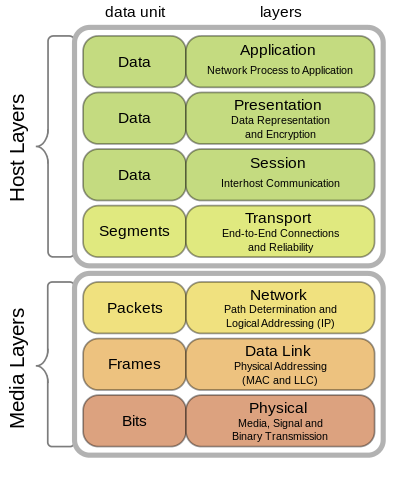
\includegraphics[scale=0.7]{pics/OSI_Model.eps}
\end{center}

\subsection{TLS}
Transport Layer Security
\begin{itemize}
	\item set of cryptographic protocols
	\item operates on layer 6 of OSI stack (Presentation Layer) (or 5? 4? 7? none? all?)
	\item independent of HTTP
	\item RFC5246 (TLS 1.2)
	\item TLS 1.3 in the works {\tt https://tools.ietf.org/html/draft-ietf-tls-tls13}
\end{itemize}
\addvspace{.5in}
Two distinct security mechanisms:
\begin{enumerate}
	\item encryption of data in transit
	\item authentication of parties
\end{enumerate}

\subsection{TLS}
Protocol:
\begin{itemize}
	\item Client Hello, present list of supported cipher suites
	\item Server Hello, chosen cipher suite
	\item Server Certificate
	\item (Server Key Exchange Message), (Client Certificate Request), (Client Certificate)
	\item Client Key Exchange Message
	\item (Certificate Verify)
	\item (Client Change Cipher Spec), (Server Change Cipher Spec)
\end{itemize}

\subsection{TLS}
\begin{center}
	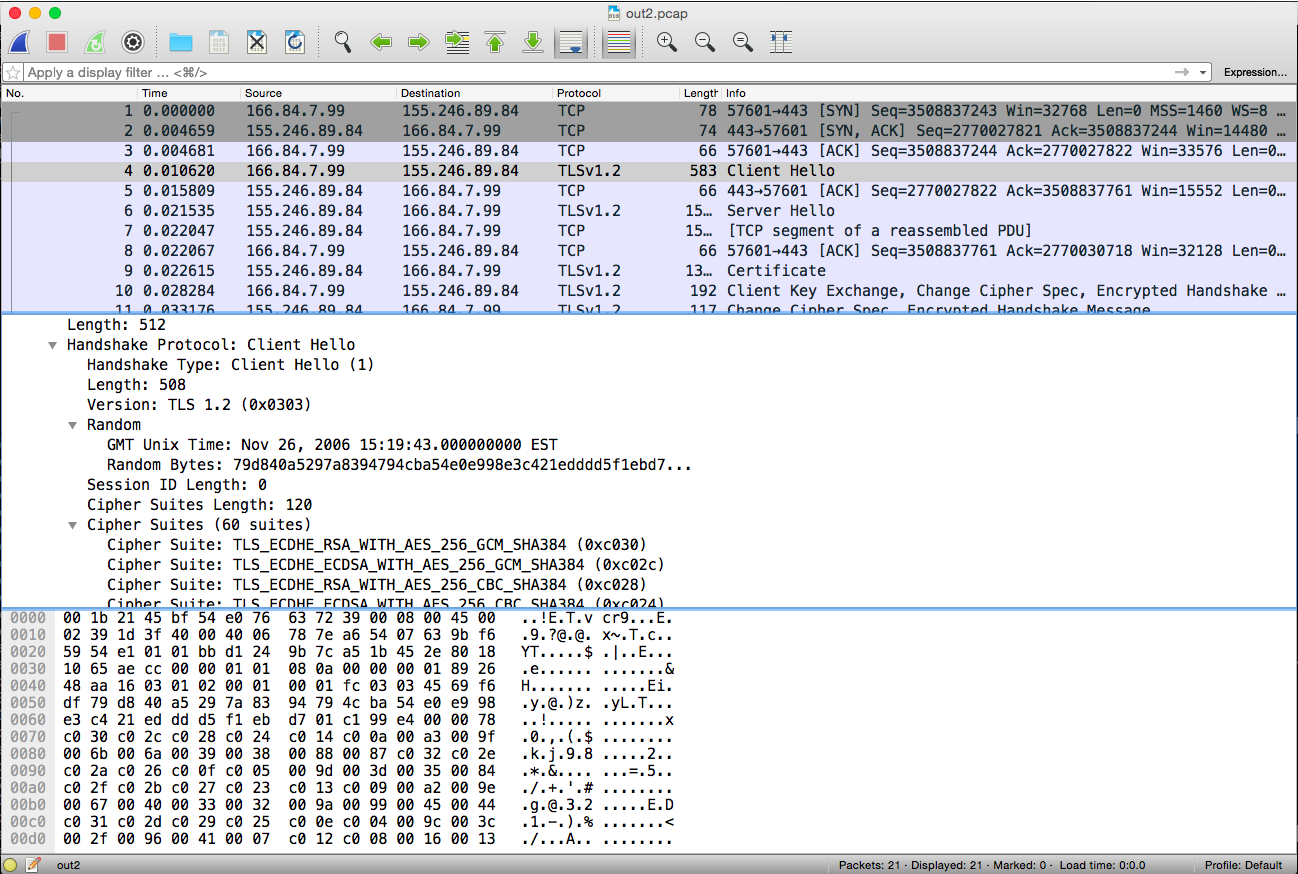
\includegraphics[scale=0.4]{pics/wireshark.eps}
\end{center}

\subsection{TLS}
\begin{verbatim}
$ openssl s_client -connect www.cs.stevens.edu:443
[...]
New, TLSv1/SSLv3, Cipher is DHE-RSA-AES256-SHA
Server public key is 2048 bit
Secure Renegotiation IS supported
Compression: NONE
Expansion: NONE
SSL-Session:
    Protocol  : TLSv1
    Cipher    : DHE-RSA-AES256-SHA
    Session-ID: 5F8A9B7A93EF87009EFCC17BBD68938C56EAACD9DF4C3643EF034D047C9F44C9
    Session-ID-ctx: 
    Master-Key: 20CBA1E477A8B573F29759045329EF7AA38C763C4C41606A46FBCC824C3F32F708789311E7B4275470E35CF09518FDCD
    Key-Arg   : None
    Start Time: 1460395966
    Timeout   : 300 (sec)
    Verify return code: 0 (ok)
\end{verbatim}

\subsection{TLS}
\smallish
\begin{verbatim}
$ openssl s_client -connect www.cs.stevens.edu:443 | \
        openssl x509 -text -noout
[...]
        Signature Algorithm: sha256WithRSAEncryption
        Issuer: C=US, ST=MI, L=Ann Arbor, O=Internet2, OU=InCommon, CN=InCommon RSA Server CA
        Validity
            Not Before: Mar  3 00:00:00 2017 GMT
            Not After : Mar  2 23:59:59 2020 GMT
        Subject: C=US/postalCode=07030, ST=NJ, L=Hoboken/street=1 Castle Point on Hudson, O=Stevens Institute of Technology, OU=IT, CN=www.cs.stevens.edu
        Subject Public Key Info:
            Public Key Algorithm: rsaEncryption
            RSA Public Key: (2048 bit)
[...]
            X509v3 Subject Alternative Name: 
                DNS:www.cs.stevens.edu, DNS:rcs.srcit.stevens.edu, DNS:svn.srcit.stevens.edu,
                DNS:www.srcit.stevens.edu
\end{verbatim}
\Normalsize
Note the absence of 'stevens-tech.edu' names...

% \subsection{TLS}
% Setting up a Man in the Middle attack site: \\
% 
% 1. start instance \\
% 
% 2. {\tt openssl req -x509 -nodes -days 30 -sha256 \
%         -newkey rsa:4096 -keyout mycert.pem -out mycert.pem}
% 
% 3. {\tt sudo openssl s\_server -WWW -accept 443 -cert mycert.pem} \\
% 
% 4. {\tt curl https://www.stevens.edu/sit/ > index.html} \\
% 
% 4. go to {\tt https://<instance>/} \\
 
\subsection{TLS Authentication}
Use of X.509:
\begin{itemize}
	\item public key certificates
	\item certificate revocation lists (CRLs) / Online Certificate Status Protocol (OCSP)
	\item certificate path validation under a Public Key Infrastructure (PKI)
	\item certificate chains depend on trust anchors
\end{itemize}

\subsection{TLS}
1. User / Company generates a {\em Certificate Signing Request} (CSR),
containing:

\begin{itemize}
	\item identifying information (distinguished name etc.)
	\item signature of data by private key
	\item chosen public key
\end{itemize}

\subsection{TLS}
1. User / Company generates a {\em Certificate Signing Request} (CSR) \\

2. CSR submitted to Certificate Authority (CA) \\

\subsection{TLS}
1. User / Company generates a {\em Certificate Signing Request} (CSR) \\

2. CSR submitted to Certificate Authority (CA) \\

3. CA verifies information \\

\subsection{TLS}
1. User / Company generates a {\em Certificate Signing Request} (CSR) \\

2. CSR submitted to Certificate Authority (CA) \\

3. CA verifies information \\

4. CA returns certificate signed with its private key \\

\subsection{TLS}
1. User / Company generates a {\em Certificate Signing Request} (CSR) \\

2. CSR submitted to Certificate Authority (CA) \\

3. CA verifies information \\

4. CA returns certificate signed with its private key \\

5. clients can verify signatures against trusted {\em root CAs} \\

\subsection{TLS}
\begin{center}
	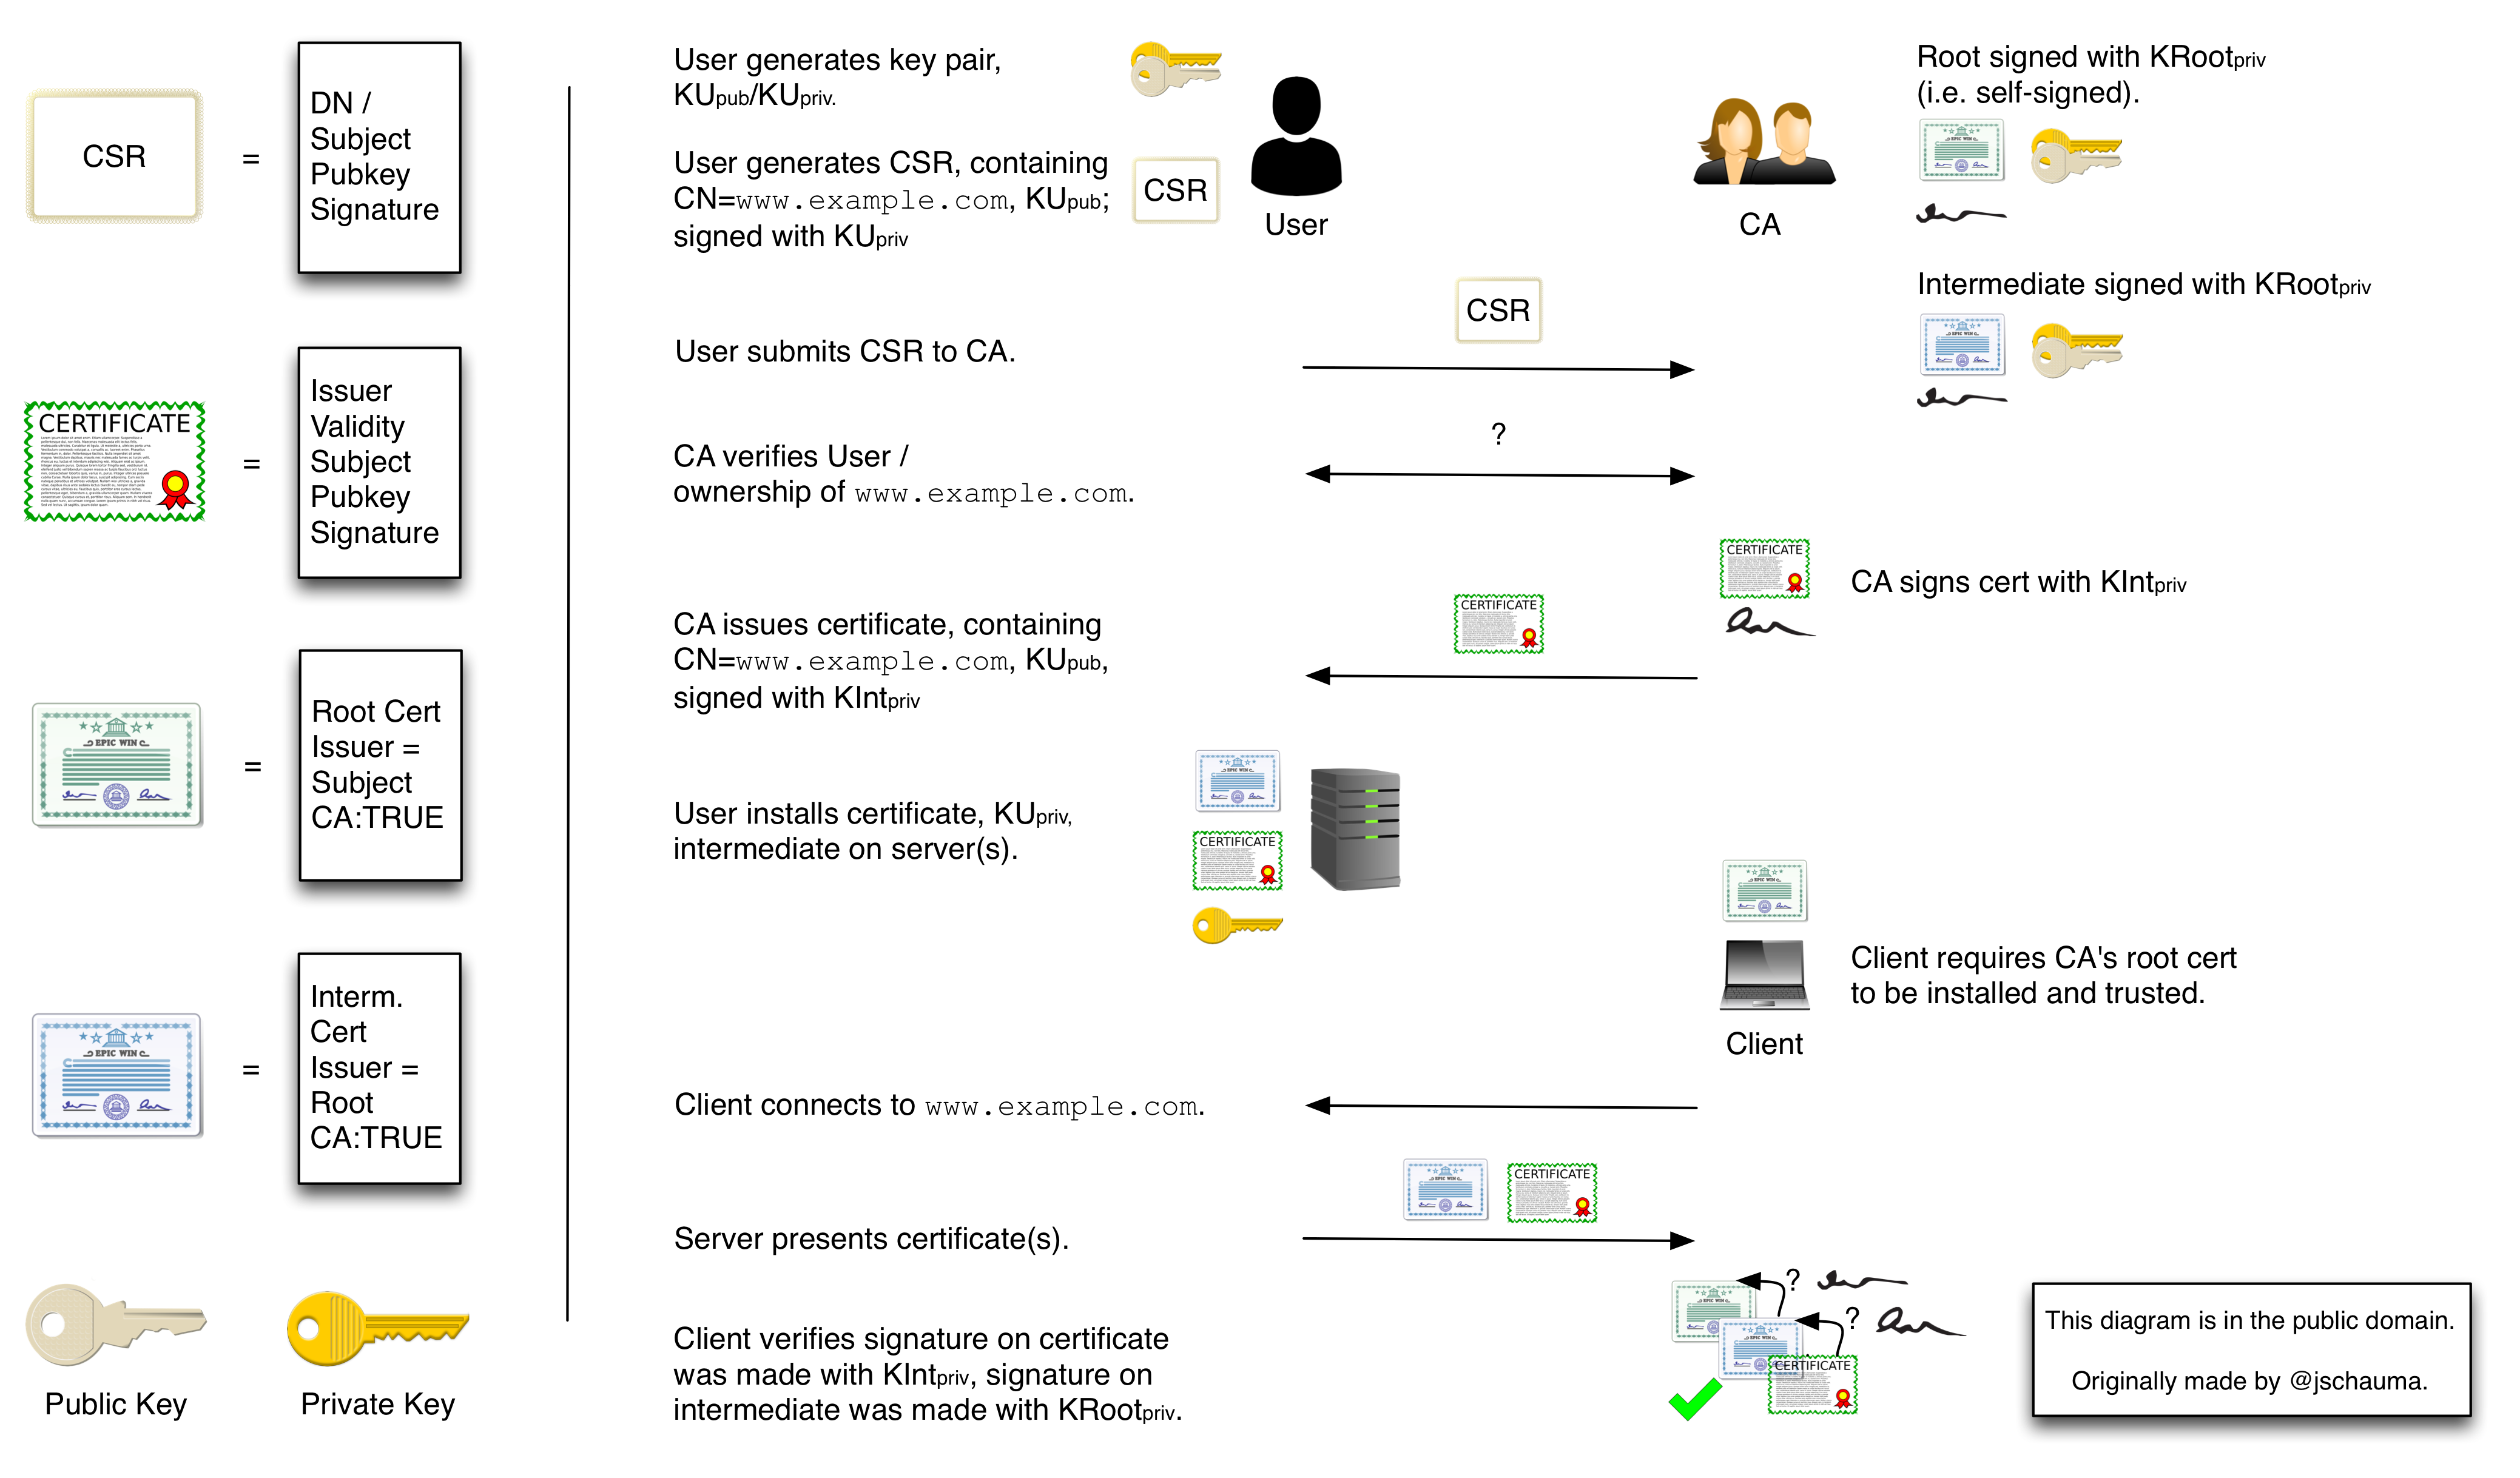
\includegraphics[scale=0.57]{pics/csr-process.eps}
\end{center}



\subsection{TLS Pitfalls}
\begin{center}
	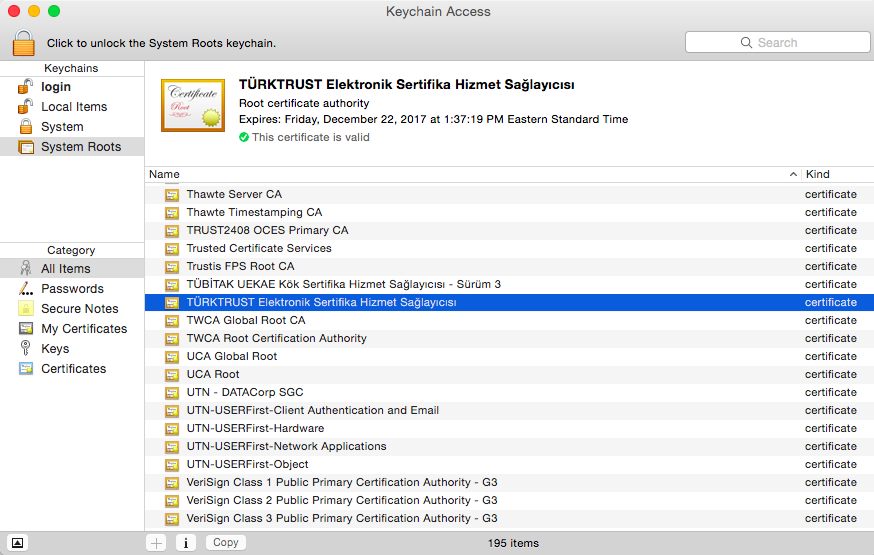
\includegraphics[scale=0.6]{pics/roots.eps} \\
	195 root CAs on this laptop...
\end{center}

\subsection{TLS Pitfalls}
Just because a site has a valid certificate does not
mean it's a trustworthy site. \\

\begin{verbatim}
https://facebook6782.webnode.com/contact/

https://vizoluh.tk/.memos/mnt/21aa3f930a55d63e6ea1eb19819c4a1a/

https://villaggioinsicilia.com/wp-includes/SimplePie/HTTP/yahoo.htm

\end{verbatim}

Do NOT submit data here!


\subsection{TLS Pitfalls}
Lack of universal HTTPS exposes users to significant
risks; many sites don't understand the importance of
authentication and encryption for non-sensitive content. \\

\verb+https://is.gd/ghiOhU+ \\

Middle boxes, often advertized as a security
mechanism, are actively harmful to users and prohibit
secure protocol development. \\

In order to serve content, you need to have the
private key $ => $ privkey available at perimeter and
exposed, high-risk systems. \\

Rotation/renewal of keys requires routine processes,
which may further expose the private key. \\

Control of a CA or a CA's key grants you near
universal powers. \\


\subsection{TLS Pitfalls}
Complex protocols, buggy implementations, intentional
weaknesses and backwards compatibility are just the
high level points.

\begin{itemize}
	\item SSLv2 obsoleted in 1996; 2016: DROWN attack
	\item SSLv3 obsoleted in 1999; 2014: POODLE attack
	\item BEAST, CRIME, BREACH, HEARTBLEED, GotoFail...
	\item obsolete and broken algorithms widely used (RC4, MD5, SHA1, ...)
\end{itemize}

\subsection{TLS}
Additional related topics:
\begin{itemize}
	\item HSTS and TLS stripping attacks
	\item HPKP and Trust On First Use (TOFU)
	\item Certificate Transparency
	\item Content Security Policy (CSP)
	\item ``Secure'' cookies vs. HttpOnly cookies
	\item attacks on domain name registrars
\end{itemize}
\addvspace{.5in}
Security is difficult.  More on that in a future
lecture.

\subsection{Reading}
SMTP
\begin{itemize}
	\item SMTP: {\tt https://tools.ietf.org/html/rfc5321}
	\item Message format: {\tt https://tools.ietf.org/html/rfc5322}
	\item SPF: {\tt https://tools.ietf.org/html/rfc7208}
	\item DKIM: {\tt https://is.gd/VnCO9f}, {\tt https://tools.ietf.org/html/rfc6376}
	\item DMARC: {\tt https://tools.ietf.org/html/rfc7489}
\end{itemize}

\subsection{Reading}
HTTPS / TLS:
\begin{itemize}
	\item {\tt https://en.wikipedia.org/wiki/HTTPS}
	\item RFC5246 (TLS 1.2) and RFC6176 (prohibiting SSL)
	\item {\tt https://bugzilla.mozilla.org/show\_bug.cgi?id=647959}
	\item {\tt https://cabforum.org}
	\item {\tt https://jhalderm.com/pub/papers/interception-ndss17.pdf}
	\item {\tt https://github.com/tlswg/tls13-spec}
	\item {\tt https://tools.ietf.org/html/draft-ietf-tls-tls13-26}
	\item {\tt https://www.imperialviolet.org/2018/03/10/tls13.html}
\end{itemize}

\end{document}
